\documentclass[12pt]{article}
\usepackage{amsfonts,amsthm,amsmath,amssymb,mathtools}
\usepackage{mathrsfs}
\usepackage{enumitem}
\usepackage{tikz-cd}
\usepackage{geometry}
\usepackage{mlmodern}

\geometry{letterpaper, portrait, margin=1in}

\setcounter{section}{0}

\renewcommand{\thesection}{\S\arabic{section}}
\renewcommand{\thesubsection}{\arabic{section}}

\newtheorem{thm}{Theorem}
\newenvironment{theorem}[1]{
	\renewcommand{\thethm}{#1}
	\begin{thm}
		}{\end{thm}}

\newtheorem{lma}{Lemma}
\newenvironment{lemma}[1]{
	\renewcommand{\thelma}{#1}
	\begin{lma}
		}{\end{lma}}

\theoremstyle{definition}
\newtheorem{ex}{Exercise}
\newenvironment{exercise}[1]{
	\renewcommand{\theex}{#1}
	\begin{ex}
		}{\end{ex}}

\title{Homework 1}
\author{Connor Mooneyhan}
\date{January 22, 2026}

\begin{document}

\maketitle

\begin{ex}
	On $\mathbb{R}^2$, let $d : X \times X \to \mathbb{R}$ be the box metric.
	Sketch the ball $B_r(x_0)$ where $x_0$ is a point in $\mathbb{R}^2$ and $r > 0$ is a real number.
	Do the same for $\mathbb{R}^3$.
\end{ex}
\begin{proof}
	I left out the axes on the second one because it was already crowded enough.
	The one on the left is an open square with side lengths 2 (where I've chosen $r = 1$), and the one on the right is a general open cube with side lengths $2r$.
	Both have $x_0$ in the center.
	\\
	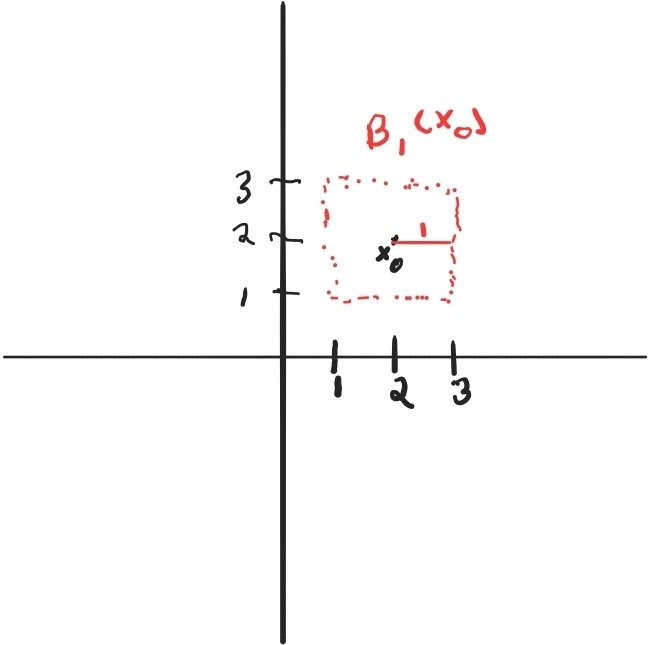
\includegraphics[width=0.5\textwidth]{2-box}
	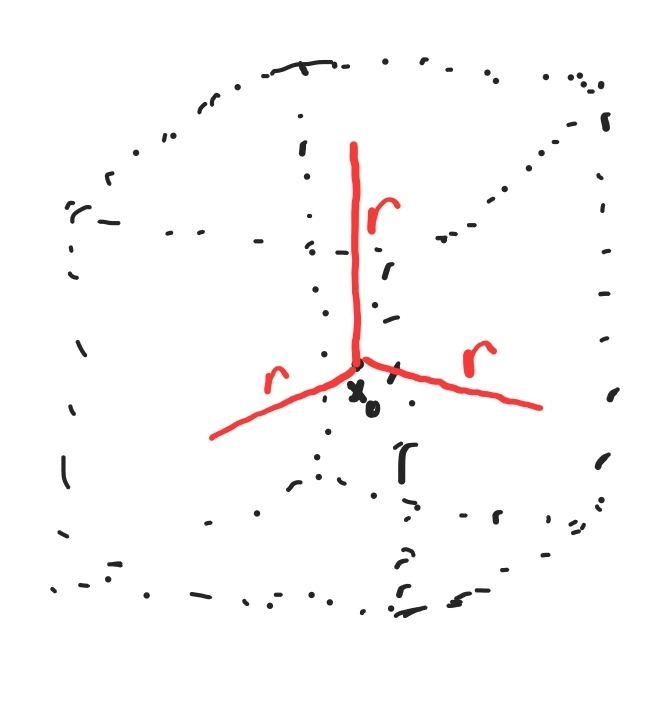
\includegraphics[width=0.5\textwidth]{3-box}
\end{proof}

\begin{ex}
	On $\mathbb{R}$, is $d(x, y) = \sqrt{|x-y|}$ a metric?
\end{ex}
\begin{proof}
	Positivity is guaranteed because we are taking principal square roots of nonnegative values $|x - y|$, and definiteness is guaranteed because \begin{equation*}
		\sqrt{|x-y|} \implies |x-y| = 0 \implies x-y = 0 \implies x = y.
	\end{equation*}
	The definition is inherently symmetric since $|x-y| = |y-x|$.
	Now assume we have $x, y, z \in \mathbb{R}$.
	Then $\sqrt{|x-z|} \leq \sqrt{|x-y| + |y-z|}$ by the triangle inequality for absolute value, and \begin{align*}
		     & \sqrt{|x-y| + |y-z|} \leq \sqrt{|x-y|} + \sqrt{|y-z|}                               \\
		\iff & \left(\sqrt{|x-y| + |y-z|}\right)^2 \leq \left(\sqrt{|x-y|} + \sqrt{|y-z|}\right)^2 \\
		\iff & |x-y| + |y-z| \leq |x-y| + 2\sqrt{|x-y||y-z|} + |y-z|                               \\
		\iff & 0 \leq 2\sqrt{|x-y||y-z|}.
	\end{align*}
	Since the last line is always true, the first line is also true, which implies that \begin{equation*}
		d(x, z) \leq d(x, y) + d(y, z).
	\end{equation*}
	Thus $d$ is a metric.
\end{proof}

\begin{ex}
	Let $X$ be the set of all ordered $n$-tuples of zeroes and ones.
	In other words, $X = \lbrace 0, 1 \rbrace^n$.
	Define \begin{equation*}
		d(x, y) = \text{ number of places where $x$ and $y$ have different entries.}
	\end{equation*}
	Show that this is a metric on $X$.
	This metric is knows as the Hamming distance and plays an important role in switching and automata theory and coding.
\end{ex}
\begin{proof}
	The phrase ``the number of'' takes care of positivity.
	If $d(x, y) = 0$, then $x$ and $y$ differ in zero entries, so they are equal, and thus $d$ is definite.
	The definition of $d$ is also inherently symmetric since the number of different entries does not change if we switch the order in which we compare the entries of $x$ and $y$.

	Now, if we have $x, y, z \in X$, then suppose the set of entries in which $x$ is different from $y$ is disjoint from the set of entries in which $y$ and $z$ are different.
	Then $d(x, z) = d(x, y) + d(y, z)$.
	If the aforementioned sets overlap, then $d(x, z) \leq d(x, y) + d(y, z)$.
	In either case, we have $d(x, z)$ is at most $d(x, y) + d(y, z)$, so the triangle inequality holds, and $d$ is indeed a metric.
\end{proof}

\begin{ex}
	Let $(X, d)$ be a metric space.
	For any non-empty subset $A \subset X$, define the \textit{diameter} of $A$ as \begin{equation*}
		\delta(A) = \sup_{x, y \in A} d(x, y).
	\end{equation*}
	A set $A$ is called bounded if $\delta(A) < \infty$.
	Show that if $A \subset B$ then $\delta(A) \leq \delta(B)$.
	Also, give an example of a metric space and two sets $A \subsetneq B$ with $\delta(A) = \delta(B)$.
\end{ex}
\begin{proof}
	If $A \subset B$, then $\lbrace d(x, y) \rbrace_{x,y \in A} \subset \lbrace d(x, y) \rbrace_{x,y \in B}$, so since $\delta(B)$ is an upper bound of the latter set, it is an upper bound of the former, and thus $\delta(A) \leq \delta(B)$ since $\delta(A)$ is the \textit{least} such upper bound.

	Now consider the trivial/discrete metric on $\mathbb{R}$, and let $A = (-1, 1)$ and $B = (-2, 2)$.
	Then we have $A \subsetneq B$ and $\delta(A) = \delta(B) = 1$.
\end{proof}

\begin{ex}
	On any metric space $X$, prove that $\delta(A) = 0$ if and only if $A$ consists of a single point.
\end{ex}
\begin{proof}
	If $\delta(A) = 0$, then the positivity of $d$ tells us that we must have $d(x, y) = 0$ for all $x, y \in A$, and definiteness guarantees that any such pair satisfies $x = y$, so $A$ consists of one point. On the other hand, if $A$ consists of a single point $x$, then indeed \begin{equation*}
		\delta(A) = \sup_{x, y \in A} d(x, y) = \sup \lbrace d(x, x) \rbrace = \sup \lbrace 0 \rbrace = 0.
	\end{equation*}
\end{proof}

\begin{ex}
	Let $(X, d_X)$, $(Y, d_Y)$ be two metric spaces.
	On the Cartesian product $X \times Y$, define, for $\mathbf{x}_1 = (x_1, y_1)$ and $\mathbf{x}_2 = (x_2, y_2)$, \begin{equation*}
		d(\mathbf{x}_1, \mathbf{x}_2) = \max(d_X(x_1, x_2), d_Y(y_1, y_2)).
	\end{equation*}
	Show that $d$ is a metric on $X \times Y$.
\end{ex}
\begin{proof}
	Since $d(\mathbf{x}_1, \mathbf{x}_2) \geq d_X(x_1,x_2) \geq 0$, we have positivity of $d$.
	Similarly, if $d(\mathbf{x}_1, \mathbf{x}_2) = 0$, then both $d_X(x_1,x_2)$ and $d_Y(y_1,y_2)$ must be 0, which implies that $x_1=x_2$ and $y_1=y_2$, so $\mathbf{x}_1 = \mathbf{x}_2$.
	By the symmetry of $d_X$ and $d_Y$, \begin{equation*}
		d(\mathbf{x}_1, \mathbf{x}_2) = \max(d_X(x_1, x_2), d_Y(y_1, y_2)) = \max(d_X(x_2, x_1), d_Y(y_2, y_1)) = d(\mathbf{x}_2, \mathbf{x}_1).
	\end{equation*}

	I'll change notations for the triangle inequality.
	Let $x = (x_1, x_2)$, $y = (y_1, y_2)$, and $z = (z_1, z_2)$.
	Then \begin{align*}
		d(x, z) & = \max(d_X(x_1, z_1), d_Y(x_2, z_2))                                         \\
		        & \leq \max(d_X(x_1, y_1) + d_X(y_1, z_1), d_Y(x_2, y_2) + d_Y(y_2, z_2))      \\
		        & \dots                                                                        \\
		        & \leq \max(d_X(x_1, y_1), d_Y(x_2, y_2)) + \max(d_X(y_1, z_1), d_Y(y_2, z_2)) \\
		        & = d(x, y) + d(y, z)
	\end{align*}
  where the third line follows from the positivity of $d_X$ and $d_Y$.
  Thus $d$ is a metric.
\end{proof}

\end{document}
